\documentclass[12pt]{article}
\usepackage[UTF8]{ctex}
\usepackage[margin=1in]{geometry}
\usepackage{graphicx} % For including figures
\usepackage{amsmath}  % For math fonts, symbols and environments
\usepackage{pgfgantt} % For Gantt charts
\usepackage[hidelinks]{hyperref} % For hyperlinks
\usepackage{enumitem} % For customizing lists
\definecolor{blue}{HTML}{74BBC9}
\definecolor{yellow}{HTML}{F7E967}
\usepackage{listings}
\usepackage{xcolor}
\usepackage{tocloft} % 导入tocloft包
\usepackage{zi4}
\usepackage{fontspec}

\usepackage{graphicx} % For including graphics
\usepackage{booktabs} % For professional looking tables
\usepackage{array}    % For extended column definitions
\usepackage{amsmath}  % For math environments like 'equation'
\usepackage{amsfonts} % For math fonts like '\mathbb{}'
\usepackage{amssymb}  % For math symbols
\usepackage{caption}  % For custom captions
\usepackage[table]{xcolor} % For coloring tables

% Set page margins
\usepackage[margin=1in]{geometry}

% 目录标题样式定义
\renewcommand{\cfttoctitlefont}{\hfill\Large\bfseries}
\renewcommand{\cftaftertoctitle}{\hfill\mbox{}\par}

% Monokai theme with a lighter background
\definecolor{codegreen}{rgb}{0,0.6,0}
\definecolor{codegray}{rgb}{0.5,0.5,0.5}
\definecolor{codepurple}{rgb}{0.58,0,0.82}
\definecolor{backcolour}{rgb}{0.95,0.95,0.92}
\setmonofont{Source Code Pro}[Contextuals={Alternate}]

\lstdefinestyle{mystyle}{
    backgroundcolor=\color{backcolour},   
    commentstyle=\color{codegreen},
    keywordstyle=\color{magenta},
    numberstyle=\tiny\color{codegray},
    stringstyle=\color{codepurple},
    basicstyle=\ttfamily\footnotesize,
    breakatwhitespace=false,         
    breaklines=true,                 
    captionpos=b,                    
    keepspaces=true,                 
    numbers=left,                    
    numbersep=5pt,                  
    showspaces=false,                
    showstringspaces=false,
    showtabs=false,                  
    tabsize=2
}

\lstset{style=mystyle}




\title{\textbf{ML第二次实验报告}}
\author{58122204 谢兴}
\date{\today}

\begin{document}


\begin{titlepage}
  \centering
  \vspace*{60pt}
  \Huge\textbf{机器学习实验报告}

  \vspace{100pt}
  \Large
  实验名称:建立全连接神经网络

  \vspace{25pt}
  学生:谢兴

  \vspace{25pt}
  学号:58122204

  \vspace{25pt}
  日期:2024/4/24

  \vspace{25pt}
  指导老师:刘胥影

  \vspace{25pt}
  助教:田秋雨



\end{titlepage}


\newpage
\tableofcontents


\section{任务描述}
通过两种方式实现全连接神经网络,并对图片分类任务行进行测试与实验。
\begin{enumerate}
  \item 手动实现简单的全连接神经网络
  \item 使用Pytorch库简洁实现全连接神经网络
\end{enumerate}

Fashion-MNIST图片分类数据集包含10个类别的时装图像,训练集有60,000张图片,测试集中有10,000张图片。图片为灰度图片,高度(h)和宽度(w)均为28像素,通道数(channel)为1。10个类别分别为:t-shirt(T恤), trouser(裤子), pullover(套衫), dress(连衣裙), coat(外套), sandal(凉鞋),shirt(衬衫),sneaker(运动鞋),bag(包),ankle boot(短靴)。使用训练集数据进行训练,测试集数据进行测试。
\section{教学要求}
\begin{enumerate}
  \item 掌握多层前馈神经网络及BP算法的原理与构建
  \item 了解PyTorch库,掌握本实验涉及的相关部分
  \item 进行参数分析实验,理解学习率等参数的影响
\end{enumerate}

\section{实验要求}
\subsection{使用Python编程构建手动实现单隐层全连接神经网络}

\textbf{模型架构}
\begin{itemize}
  \item 输入层 \( 28 \times 28 = 784 \) 个节点,输出层10个节点,隐藏层256个节点。注意,可以将这两个变量都视为超参数。通常选择2的若干次幂作为层的宽度。因为内存在硬件中的分配和寻址方式,这么做往往可以在计算上更高效。
  \item 激活函数:ReLU函数
  \item 损失函数:Cross entropy
  \item 性能指标:准确率
  \item 优化算法:实现标准BP或小批量梯度下降算法均可
\end{itemize}

\textbf{实现内容}
\begin{enumerate}
  \item 初始化模型参数:对于每一层都要记录一个权重矩阵和一个偏置向量。
  \item 设置激活函数:使用ReLU函数作为激活函数,要求手动实现该函数。
  \item 前向计算:实现该函数。注意:需要将每个二维图像转化为向量进行操作。
  \item 设置损失函数:使用cross entropy作为损失函数。可以自己手动实现,也可以直接调用\texttt{nn.CrossEntropyLoss}函数。
  \item 训练模型:
        \begin{enumerate}
          \item 实现训练函数:该训练函数将会运行多个迭代周期(由\textit{num\_epochs}指定)。在每个迭代周期结束时,利用\textit{test\_iter}访问到的测试数据集对模型进行评估。利用后面给出的Animator类来可视化训练进度。
          \item 可以使用PyTorch内置的优化器(\texttt{torch.optim.SGD}),也可以使用自己定制的优化器。
          \item 可以调用\texttt{torch.optim.SGD}函数进行参数更新。
          \item 迭代周期数\textit{epoch}设置为10,学习率设置为0.1,训练模型。
        \end{enumerate}
  \item 设置性能函数:使用准确率\textit{accuracy}作为性能指标。实现该函数。
  \item 模型评估:
        \begin{enumerate}
          \item 对测试集数据进行测试。
          \item 进行性能评估。
        \end{enumerate}
  \item 参数分析实验:
        \begin{enumerate}
          \item 在所有其他参数保持不变的情况下,更改超参数\textit{num\_hiddens}的值,并查看此超参数的变化对结果有何影响。确定此超参数的最佳值。
          \item 改变学习速率会如何影响结果?保持模型架构和其他超参数(包括轮数)不变,学习率设置为多少会带来最好的结果?
        \end{enumerate}
\end{enumerate}

\subsection{使用PyTorch库简洁实现全连接神经网络}

手动实现一个简单的多层神经网络是很容易的。然而如果网络有很多层,从零开始实现会变得很麻烦。可以使用高级API如PyTorch库简洁实现。


\begin{enumerate}
  \item 请使用PyTorch库简洁实现前述的全连接神经网络,并进行模型评估。
        \begin{enumerate}
          \item 优化器:使用\texttt{torch.optim.SGD}
          \item 小批量数据载入函数参见提供的代码。
        \end{enumerate}
  \item \textbf{参数分析实验}
        \begin{enumerate}
          \item 尝试添加不同数量的隐藏层(也可以修改学习率),怎么样设置效果最好?
          \item 尝试不同的激活函数,哪个效果最好?
          \item 尝试不同的方案来初始化权重,什么方法效果最好?
        \end{enumerate}
\end{enumerate}

\subsection{提交要求}
其中报告内容包括以下几个部分:
\begin{enumerate}
  \item 手动实现单隐层全连接神经网络
        \begin{enumerate}
          \item 训练过程中,训练集与验证集误差随epoch变化的曲线图
          \item 性能评估结果
          \item 参数分析实验:包括实验设置与结果分析
        \end{enumerate}
  \item 使用PyTorch库简洁实现全连接神经网络
        \begin{enumerate}
          \item 性能评估结果
          \item 参数分析实验:包括实验设置与结果分析
        \end{enumerate}
\end{enumerate}



\section{实验部分}
\subsection{实验环境}
实验环境见表~\ref{tab:indicators}。

\begin{table}[!t]
  \caption{Experiment Environment}
  \label{tab:indicators}
  \centering
  \begin{tabular}{m{5cm}<{\centering}m{5cm}<{\centering}m{4cm}<{\centering}}
    \toprule
    \textbf{Items}   & \textbf{Version}     \\[\medskipamount]
    \midrule
    CPU              & Intel Core i5-1135G7 \\[\medskipamount]
    RAM              & 16 GB                \\[\medskipamount]
    Python           & 3.11.5               \\[\medskipamount]
    Pytorch          & 2.2.1                \\[\medskipamount]
    Operating system & Windows11            \\[\medskipamount]
    \bottomrule
  \end{tabular}
\end{table}


\subsection{使用Python编程构建手动实现单隐层全连接神经网络}
\subsubsection{模型训练参数与可视化}

\begin{enumerate}
  \item 输入层28*28=784个节点,输出层10个节点,隐藏层256个节点
  \item 激活函数:ReLU函数
  \item 损失函数:Cross entropy
  \item 性能指标:准确率
  \item 小批量梯度下降算法
\end{enumerate}

\textbf{训练过程可视}

如图~\ref{1_1} 和图~\ref{1_2} 所示。
(囿于实验环境算力有限,训练过程可视化没有实现测验集误差和准确率随batch的变化曲线)
\begin{figure}[htbp]
  \centering
  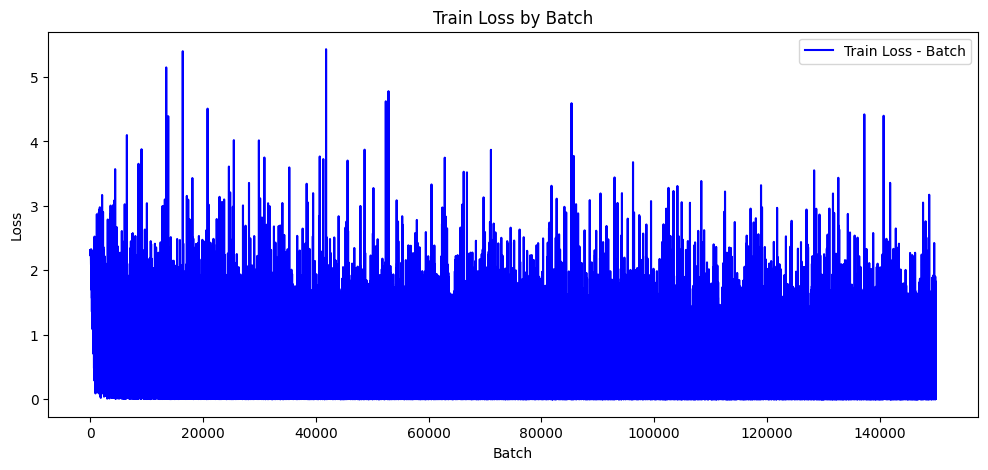
\includegraphics[width=0.8\textwidth]{1_1.png}
  \caption[训练集误差随batch变化的曲线图]{训练集误差随batch变化的曲线图}
  \label{1_1}
\end{figure}

\begin{figure}[htbp]
  \centering
  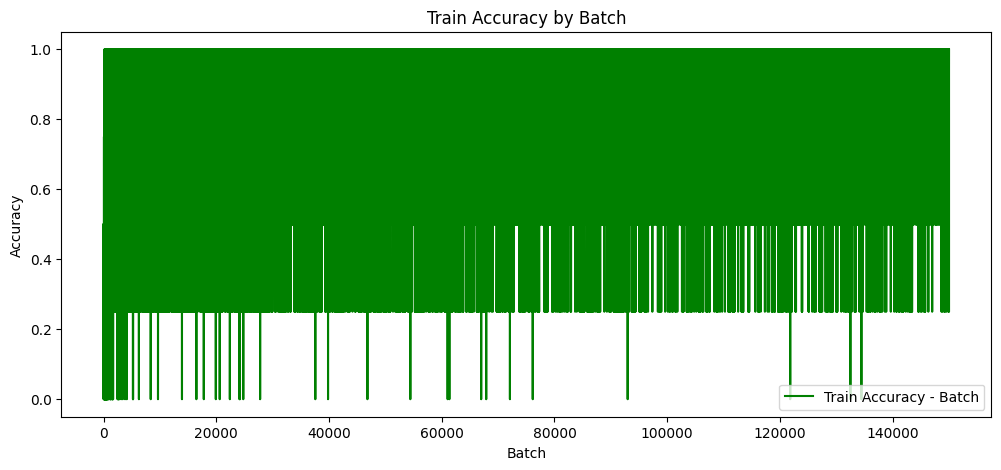
\includegraphics[width=0.8\textwidth]{1_2.png}
  \caption[训练集准确率随batch变化的曲线图]{训练集准确率随batch变化的曲线图}
  \label{1_2}
\end{figure}

\subsubsection{模型评估与实验结果}
训练过程中,训练集与验证集误差随epoch变化的曲线图如图~\ref{1_3} 所示。从图中可以看到模型经过10个epoch的迭代,从图中可以看到模型经过10个epoch的迭代,模型在训练集和测验集上的准确率均高于87\%,
模型在训练集和测验集上的loss均低于0.4,说明模型具有较强的分类预测能力。

但与此同时,模型在测验集上的准确率低于在训练集上的准确率,说明模型存在一定的过拟合现象。

这两者评估结果表明多层感知机的模型性能较为强大。

\begin{figure}[htbp]
  \centering
  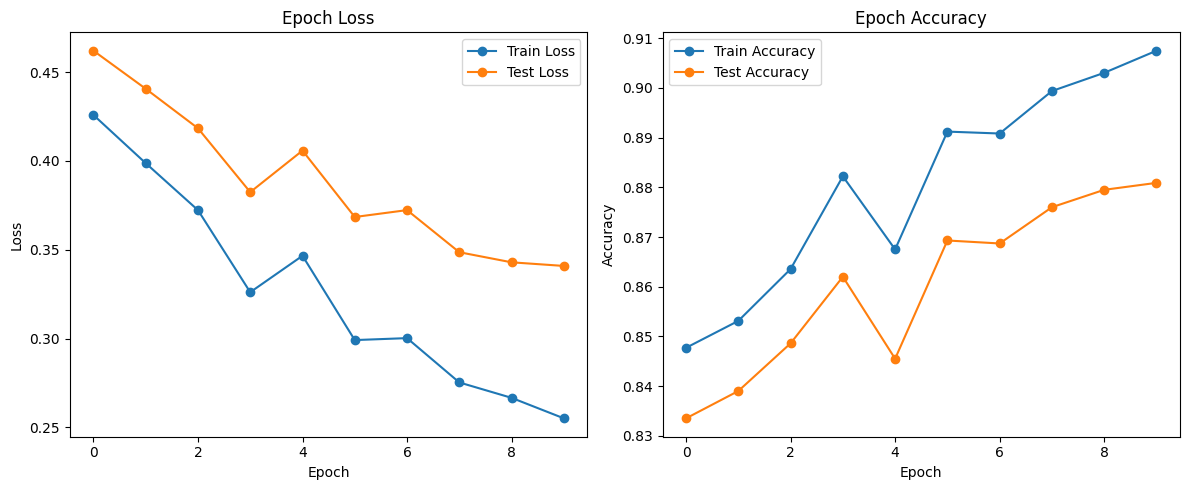
\includegraphics[width=0.8\textwidth]{1_3.png}
  \caption[训练集与验证集误差随epoch变化的曲线图]{训练集与验证集误差随epoch变化的曲线图}
  \label{1_3}
\end{figure}


\subsubsection{参数分析实验}

\begin{enumerate}
  \item \textbf{修改隐藏层数}

        分别测试了num\_hiddens为64, 128, 256, 512时的模型性能,发现num\_hiddens为256时,模型性能最好。同时我也观察到num\_hiddens越大,
        模型训练所需时间越长。
  \item \textbf{修改学习率}

        分别测试了lr为0.01, 0.05,0.1,时的模型性能,发现lr为0.01时,模型性能最好。调参过程中注意到lr越小,模型训练所需时间越长。
  \item \textbf{修改epoch}

        进过调参的经验和实际测试发现,epoch增大,模型预测的准确率会有一定的提高,但是增大到一定程度后,模型的准确率会趋于稳定,不再有明显的提高。
        并且增大epoch会增加训练时间,所以在实际应用中,需要根据实际情况来选择epoch的大小。
\end{enumerate}




\subsection{使用PyTorch库简洁实现全连接神经网络}

\subsubsection{模型训练参数与可视化}
使用PyTorch库简洁实现全连接神经网络的训练参数如表~\ref{tab:training-params} 所示。
\begin{table}[htbp]
  \centering
  \caption{训练参数}
  \label{tab:training-params}
  \begin{tabular}{m{3cm}<{\centering}m{3cm}<{\centering}}
    \toprule
    \textbf{参数}   & \textbf{值}    \\[\medskipamount]
    \midrule
    learning rate & 0.1           \\[\medskipamount]
    epochs        & 10            \\[\medskipamount]
    optimizer     & SGD           \\[\medskipamount]
    loss function & Cross Entropy \\[\medskipamount]
    performance   & accuracy      \\[\medskipamount]
    batch size    & 16            \\[\medskipamount]
    num\_hiddens  & 256            \\[\medskipamount]
    \bottomrule
  \end{tabular}
\end{table}

\textbf{训练过程可视化}

如图~\ref{2_1} 和图~\ref{2_2} 所示。
(囿于实验环境算力有限,训练过程可视化没有实现测验集误差和准确率随batch的变化曲线)
\begin{figure}[htbp]
  \centering
  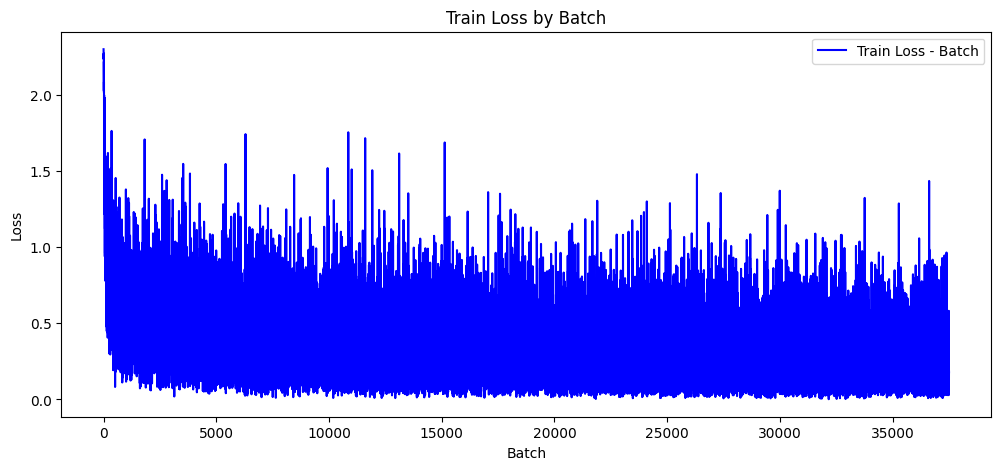
\includegraphics[width=0.8\textwidth]{2_1.png}
  \caption[训练集误差随batch变化的曲线图]{训练集误差随batch变化的曲线图}
  \label{2_1}
\end{figure}

\begin{figure}[htbp]
  \centering
  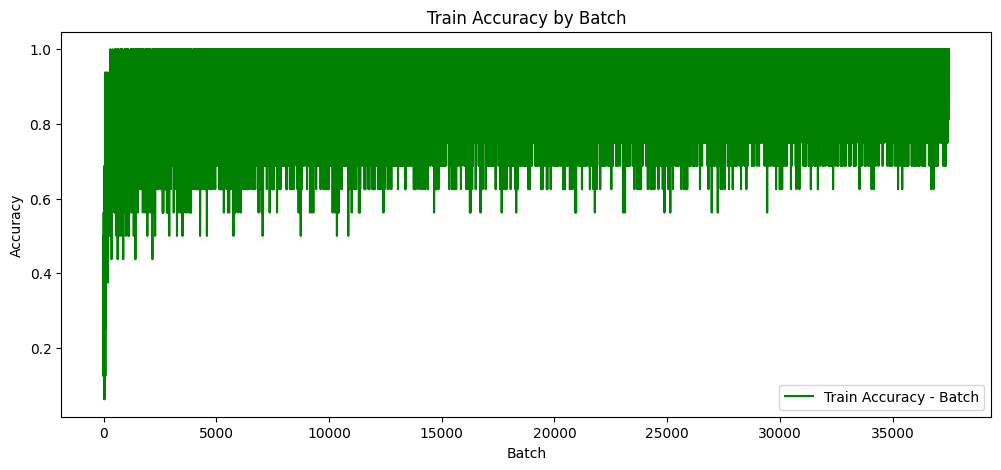
\includegraphics[width=0.8\textwidth]{2_2.png}
  \caption[训练集准确率随batch变化的曲线图]{训练集准确率随batch变化的曲线图}
  \label{2_2}
\end{figure}



\subsubsection{模型评估与实验结果}
训练过程中,训练集与验证集误差随epoch变化的曲线图如图~\ref{2_3} 所示。从图中可以看到模型经过10个epoch的迭代,模型在训练集和测验集上的准确率均高于87\%,
模型在训练集和测验集上的loss均低于0.4,说明模型具有较强的分类预测能力。

但与此同时,模型在测验集上的准确率低于在训练集上的准确率,说明模型存在一定的过拟合现象。

这两者评估结果表明多层感知机的模型性能较为强大。

\begin{figure}[htbp]
  \centering
  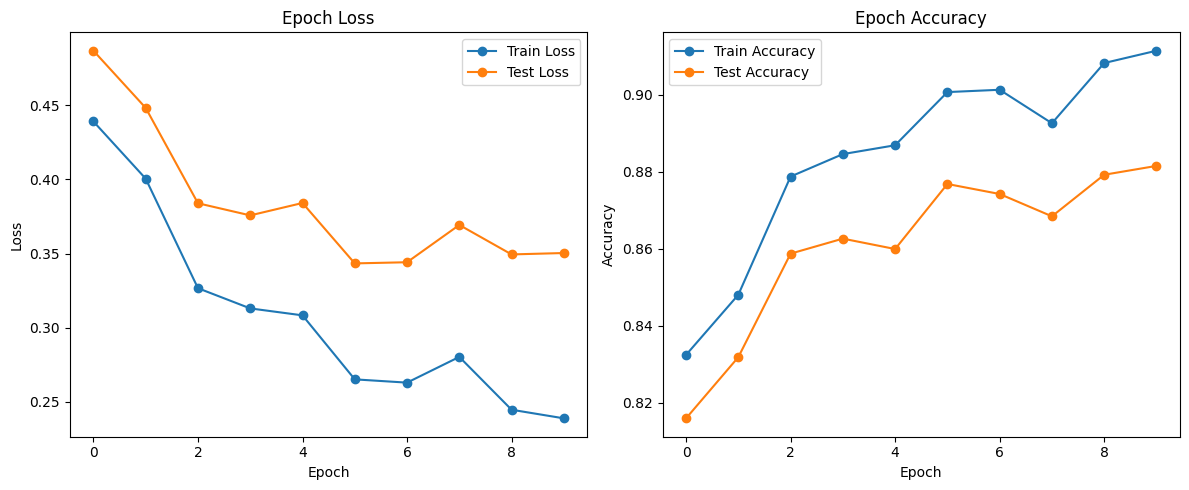
\includegraphics[width=0.8\textwidth]{2_3.png}
  \caption[训练集与验证集误差随epoch变化的曲线图]{训练集与验证集误差随epoch变化的曲线图}
  \label{2_3}
\end{figure}


\subsubsection{参数分析实验}

\begin{enumerate}
  \item \textbf{修改隐藏层数和学习率}

        分别测试了lr为0.01, 0.05,0.1,时的模型性能,发现lr为0.01时,模型性能最好。
        分别测试了num\_hiddens为64, 128, 256, 512时的模型性能,发现num\_hiddens为256时,模型性能最好。
  \item \textbf{使用不同的激活函数}

        分别使用了relu和sigmoid作为激活函数,发现relu的效果更好。
  \item \textbf{使用不同的方案来初始化权重}
         
        分别使用了不同的方案初始化权重,发现以下的参数初始化方法效果最好。
  \begin{lstlisting}
    # Initialize parameters
    nn.init.normal_(self.fc1.weight, mean=0, std=0.1)
    nn.init.constant_(self.fc1.bias, 0)
    nn.init.normal_(self.fc2.weight, mean=0, std=0.1)
    nn.init.constant_(self.fc2.bias, 0)
  \end{lstlisting}
        
\end{enumerate}


\section{实验总结}

\subsection{实验结果}
本次实验实现了两种方式的全连接神经网络,一种是手动实现的简单全连接神经网络,另一种是使用PyTorch库简洁实现的全连接神经网络。
通过实验,我们发现使用PyTorch库简洁实现的全连接神经网络在训练过程中的代码量更少,更加简洁,同时也更加高效。在参数分析实验中,
我们发现在手动实现的全连接神经网络中,隐藏层节点数为256时,效果最好;在PyTorch库简洁实现的全连接神经网络中,隐藏层节点数为256时,效果最好。

\subsection{实验感悟}
通过这次实验,我对全连接神经网络有了更深入的了解,掌握了多层前馈神经网络及BP算法的原理与构建,了解了PyTorch库,掌握了本实验涉及的相关部分。

\subsection{实验的不足以及改进方向}
\textbf{模型性能方面}:
这次实验是通过两种方式实现全连接神经网络,并对图片数据集Fashion-MNIST中的图片进行分类,我们可以看到,本次实验的准确率并不是很高(仅有85\%左右),
一方面与实验的epochs数过小有关,另一方面也与模型本身的性能有关,在以后的学习中可以使用更加复杂的模型(如CNN等),以提高模型的准确率等性能。

\textbf{训练过程可视化方面}:未来我们可以采用像YOLOv5那样在训练过程中直接在终端实时动态更新输出每一个batch后参数更新后的各种loss,和准确率,召回率,
置信度等相关参数等。

\newpage
% 开始附录部分
\appendix
% 手动添加附录到目录中
\addcontentsline{toc}{section}{附录}
\section{使用Python编程构建手动实现单隐层全连接神经网络Code}
\begin{lstlisting}[language=Python]
  import numpy as np
  import matplotlib.pyplot as plt
  from torchvision import datasets, transforms
  from torch.utils.data import DataLoader
  import config
  args = config.args
  
  
  # 数据加载
  trans = transforms.ToTensor()
  mnist_train = datasets.FashionMNIST(root="./data", train=True, transform=trans, download=True)
  mnist_test = datasets.FashionMNIST(root="./data", train=False, transform=trans, download=True)
  
  num_inputs, num_outputs, num_hiddens = 784, 10, 256
  
  
  train_iter = DataLoader(mnist_train, batch_size=args.batch_size, shuffle=True, num_workers=0)
  test_iter = DataLoader(mnist_test, batch_size=10000, shuffle=False, num_workers=0)
  
  # 激活函数和softmax函数
  def relu(x):
      return np.maximum(x, 0)
  
  def sigmoid(x):
      return 1 / (1 + np.exp(-x))

  def softmax(x):
      exp_x = np.exp(x - np.max(x, axis=1, keepdims=True))
      return exp_x / np.sum(exp_x, axis=1, keepdims=True)
  
  # 损失函数
  def cross_entropy(y_hat, y):
      m = y_hat.shape[0]
      y_one_hot = np.eye(num_outputs)[y]
      return -np.sum(np.log(y_hat[range(m), y])) / m
  
  # 前向传播
  def model(X, w1, b1, w2, b2):
      H = relu(np.dot(X, w1) + b1)
      O = np.dot(H, w2) + b2
      return softmax(O), H
  
  # 梯度计算
  def calc_gradient(X, y, y_hat, H, w2):
      m = y.shape[0]
      y_one_hot = np.eye(num_outputs)[y]
  
      dO = (y_hat - y_one_hot) / m
      grad_w2 = np.dot(H.T, dO)
      grad_b2 = np.sum(dO, axis=0)
  
      dH = np.dot(dO, w2.T) * (H > 0).astype(float)
      grad_w1 = np.dot(X.T, dH)
      grad_b1 = np.sum(dH, axis=0)
  
      return grad_w1, grad_b1, grad_w2, grad_b2
  
  # 参数更新
  def update_params(params, grads, lr):
      for param, grad in zip(params, grads):
          param -= lr * grad
  
  # 参数初始化
  w1 = np.random.randn(num_inputs, num_hiddens) * 0.01
  b1 = np.zeros(num_hiddens)
  w2 = np.random.randn(num_hiddens, num_outputs) * 0.01
  b2 = np.zeros(num_outputs)
  params = [w1, b1, w2, b2]
  
  # Metrics storage
  batch_metrics = {
      'train_losses': [], 
      'train_accs': [], 
      'test_losses': [], 
      'test_accs': []
  }
  epoch_metrics = {
      'train_losses': [], 
      'train_accs': [], 
      'test_losses': [], 
      'test_accs': []
  }
  def accuracy(loader, w1, b1, w2, b2):
      total_loss = 0
      total_correct = 0
      total_samples = 0
      
      # 设置数据加载器加载的是numpy数组而非torch.Tensor
      for images, labels in loader:
          X = images.view(-1, num_inputs).numpy()  # 转换为适当的形状和类型
          y = labels.numpy()
          
          # 前向传播
          y_hat, _ = model(X, w1, b1, w2, b2)
          
          # 计算损失
          loss = cross_entropy(y_hat, y)
          total_loss += loss * len(y)  # 累计总损失
          total_correct += (np.argmax(y_hat, axis=1) == y).sum()  # 计算正确预测的数量
          total_samples += len(y)
      
      average_loss = total_loss / total_samples
      accuracy = total_correct / total_samples
      return average_loss, accuracy
  
  # Training and evaluation loop
  
  for epoch in range(args.epochs):
      for images, labels in train_iter:
          X = images.view(-1, num_inputs).numpy()
          y = labels.numpy()
          y_hat, H = model(X, *params)
          loss = cross_entropy(y_hat, y)
          grads = calc_gradient(X, y, y_hat, H, w2)
          update_params(params, grads, lr=args.lr)
  
          batch_metrics['train_losses'].append(loss)
          batch_acc = (np.argmax(y_hat, axis=1) == y).mean()
          batch_metrics['train_accs'].append(batch_acc)
  
      # Evaluate at the end of each epoch
      epoch_train_loss, epoch_train_acc = accuracy(train_iter, *params)
      epoch_test_loss, epoch_test_acc = accuracy(test_iter, *params)
  
      epoch_metrics['train_losses'].append(epoch_train_loss)
      epoch_metrics['train_accs'].append(epoch_train_acc)
      epoch_metrics['test_losses'].append(epoch_test_loss)
      epoch_metrics['test_accs'].append(epoch_test_acc)
  
      print(f'Epoch {epoch + 1}, Train Loss: {epoch_train_loss:.6f}, Train Acc: {epoch_train_acc:.6f}, Test Loss: {epoch_test_loss:.6f}, Test Acc: {epoch_test_acc:.6f}')
  
  
  
  
  # 绘制训练和测试损失与准确率的曲线图
  
  
  # 绘制训练损失的曲线图
  plt.figure(figsize=(12, 5))
  plt.plot(batch_metrics['train_losses'], label='Train Loss - Batch', color='blue')
  plt.title('Train Loss by Batch')
  plt.xlabel('Batch')
  plt.ylabel('Loss')
  plt.legend()
  plt.show()
  
  
  # 绘制训练准确率的曲线图
  plt.figure(figsize=(12, 5))
  plt.plot(batch_metrics['train_accs'], label='Train Accuracy - Batch', color='green')
  plt.title('Train Accuracy by Batch')
  plt.xlabel('Batch')
  plt.ylabel('Accuracy')
  plt.legend()
  plt.show()
  
  
  # 绘制训练和测试损失的曲线图
  plt.figure(figsize=(12, 5))
  plt.subplot(1, 2, 1)
  plt.plot(epoch_metrics['train_losses'], label='Train Loss', marker='o')
  plt.plot(epoch_metrics['test_losses'], label='Test Loss', marker='o')
  plt.title('Epoch Loss')
  plt.xlabel('Epoch')
  plt.ylabel('Loss')
  plt.legend()
  
  # 绘制训练和测试准确率的曲线图
  plt.subplot(1, 2, 2)
  plt.plot(epoch_metrics['train_accs'], label='Train Accuracy', marker='o')
  plt.plot(epoch_metrics['test_accs'], label='Test Accuracy', marker='o')
  plt.title('Epoch Accuracy')
  plt.xlabel('Epoch')
  plt.ylabel('Accuracy')
  plt.legend()
  
  plt.tight_layout()
  plt.show()
\end{lstlisting}


\section{使用PyTorch库简洁实现全连接神经网络Code}
\begin{lstlisting}[language=Python]
  import torch
  from torch import nn, optim
  from torchvision import datasets, transforms
  from torch.utils.data import DataLoader
  import matplotlib.pyplot as plt
  import config
  
  args = config.args
  device = torch.device('cuda' if not args.cpu and torch.cuda.is_available() else 'cpu')
  
  # Data loading
  trans = transforms.ToTensor()
  mnist_train = datasets.FashionMNIST(root="./data", train=True, transform=trans, download=True)
  mnist_test = datasets.FashionMNIST(root="./data", train=False, transform=trans, download=True)
  
  # Model definition
  class CustomNetwork(nn.Module):
      def __init__(self, num_inputs, num_hiddens, num_outputs):
          super(CustomNetwork, self).__init__()
          self.fc1 = nn.Linear(num_inputs, num_hiddens)
          self.fc2 = nn.Linear(num_hiddens, num_outputs)
          # Initialize parameters
          nn.init.normal_(self.fc1.weight, mean=0, std=0.01)
          nn.init.constant_(self.fc1.bias, 0)
          nn.init.normal_(self.fc2.weight, mean=0, std=0.01)
          nn.init.constant_(self.fc2.bias, 0)
  
      def forward(self, x):
          x = torch.relu(self.fc1(x))
          x = self.fc2(x)
          return x
  
  # Model instantiation, loss, and optimizer
  model = CustomNetwork(784, 256, 10).to(device)
  criterion = nn.CrossEntropyLoss()
  optimizer = optim.SGD(model.parameters(), lr=args.lr)
  
  # Data loading
  train_loader = DataLoader(mnist_train, batch_size=args.batch_size, shuffle=True)
  test_loader = DataLoader(mnist_test, batch_size=10000, shuffle=False)
  
  # Function to evaluate the network
  def accuracy(loader):
      total_loss, total_correct, total = 0, 0, 0
      model.eval()
      with torch.no_grad():
          for images, labels in loader:
              images = images.view(-1, 784).to(device)
              labels = labels.to(device)
              output = model(images)
              loss = criterion(output, labels)
              total_loss += loss.item()
              total_correct += (output.argmax(1) == labels).sum().item()
              total += labels.size(0)
      model.train()
      return total_loss / len(loader), total_correct / total
  
  # Metrics storage
  batch_metrics = {
      'train_losses': [], 
      'train_accs': [], 
      'test_losses': [], 
      'test_accs': []
  }
  epoch_metrics = {
      'train_losses': [], 
      'train_accs': [], 
      'test_losses': [], 
      'test_accs': []
  }
  
  # Training and evaluation loop
  for epoch in range(args.epochs):
      for images, labels in train_loader:
          images = images.view(-1, 784).to(device)
          labels = labels.to(device)
          output = model(images)
          loss = criterion(output, labels)
          optimizer.zero_grad()
          loss.backward()
          optimizer.step()
  
          # Record batch loss and accuracy
          batch_loss = loss.item()
          batch_accuracy = (output.argmax(1) == labels).float().mean().item()
          batch_metrics['train_losses'].append(batch_loss)
          batch_metrics['train_accs'].append(batch_accuracy)
  
      # Evaluate on test data after each epoch
      test_loss, test_accuracy = accuracy(test_loader)
      batch_metrics['test_losses'].append(test_loss)
      batch_metrics['test_accs'].append(test_accuracy)
      
      # Record epoch metrics
      epoch_train_loss, epoch_train_acc = accuracy(train_loader)
      epoch_metrics['train_losses'].append(epoch_train_loss)
      epoch_metrics['train_accs'].append(epoch_train_acc)
      epoch_metrics['test_losses'].append(test_loss)
      epoch_metrics['test_accs'].append(test_accuracy)
  
      print(f'Epoch {epoch + 1}, Train Loss: {epoch_train_loss:.6f}, Train Acc: {epoch_train_acc:.6f}, Test Loss: {test_loss:.6f}, Test Acc: {test_accuracy:.6f}')
  
  # Plotting code
  
  # Plotting
  # 绘制训练损失的曲线图
  plt.figure(figsize=(6, 5))
  plt.plot(batch_metrics['train_losses'], label='Train Loss - Batch', color='blue')
  plt.title('Train Loss by Batch')
  plt.xlabel('Batch')
  plt.ylabel('Loss')
  plt.legend()
  plt.show()
  
  
  # 绘制训练准确率的曲线图
  plt.figure(figsize=(6, 5))
  plt.plot(batch_metrics['train_accs'], label='Train Accuracy - Batch', color='green')
  plt.title('Train Accuracy by Batch')
  plt.xlabel('Batch')
  plt.ylabel('Accuracy')
  plt.legend()
  plt.show()
  
  
  
  # 绘制训练和测试损失的曲线图
  plt.figure(figsize=(12, 5))
  plt.subplot(1, 2, 1)
  plt.plot(epoch_metrics['train_losses'], label='Train Loss', marker='o')
  plt.plot(epoch_metrics['test_losses'], label='Test Loss', marker='o')
  plt.title('Epoch Loss')
  plt.xlabel('Epoch')
  plt.ylabel('Loss')
  plt.legend()
  
  # 绘制训练和测试准确率的曲线图
  plt.subplot(1, 2, 2)
  plt.plot(epoch_metrics['train_accs'], label='Train Accuracy', marker='o')
  plt.plot(epoch_metrics['test_accs'], label='Test Accuracy', marker='o')
  plt.title('Epoch Accuracy')
  plt.xlabel('Epoch')
  plt.ylabel('Accuracy')
  plt.legend()
  
  plt.tight_layout()
  plt.show()
  
  
  args.save(model.state_dict(), 'fashion_mnist.pt')

\end{lstlisting}


\section{config.py}
\begin{lstlisting}[language=Python]

  import argparse
parser = argparse.ArgumentParser(description='Hyper-parameters management')

# Hardware options
parser.add_argument('--n_threads', type=int, default=6,
                    help='number of threads for data loading')
parser.add_argument('--cpu', action='store_true',
                    help='use cpu only')
parser.add_argument('--seed', type=int, default=1, help='random seed')

# data in/out and dataset
parser.add_argument('--dataset_path',default = './data/',help='fixed trainset root path')

parser.add_argument('--save',default='model',help='save path of trained model')

parser.add_argument('--predict',default='model',help='save path of predict model')

parser.add_argument('--batch_size', type=list, default=256,help='batch size of trainset')

# train
parser.add_argument('--epochs', type=int, default=10, metavar='N',help='number of epochs to train (default: 10)')

parser.add_argument('--lr', type=float, default=0.1, metavar='LR',help='learning rate (default: 0.01)')

parser.add_argument('--momentum', type=float, default=0.99, metavar='M',help='SGD momentum (default: 0.5)')

parser.add_argument('--weight_decay', type=float, default=3e-5, metavar='W',help='SGD weight_decay (default: 3e-5)')

parser.add_argument('--nesterov', type=bool, default=True, help='SGD nesterov (default: True)')

parser.add_argument('--early-stop', default=20, type=int, help='early stopping (default: 20)')
#args = parser.parse_args()
args, unknown = parser.parse_known_args()
  

\end{lstlisting}


\section{predict.py}



\end{document}
